\documentclass[fleqn]{beamer}

\usepackage[british]{babel}
\usepackage{graphicx,ru,url}
\usepackage{amsmath}
% Use Times for math font and text font.
\RequirePackage[T1]{fontenc}
%\RequirePackage{txfonts}
% bold math must be loaded after Times font
\usepackage{bm}
\usepackage{booktabs} % nice rules (thick lines) for tables
\usepackage{microtype} % improves typography for PDF
\usepackage{xcolor} % Allows colors in fonts
\usepackage{tikz} % Allows creation of tikz pictures
\usepackage{verbatim}
\usetikzlibrary{arrows,shapes,snakes}
\usepackage{hyperref}
% \usepackage{minted} % Allows printing of python (or other) code
% \newminted{python}{fontsize=\scriptsize, 
%     linenos,
%     numbersep=8pt,
%     gobble=4,
%     frame=lines,
%     bgcolor=bg,
%     framesep=3mm}

% The title of the presentation:
%  - first a short version which is visible at the bottom of each slide;
%  - second the full title shown on the title slide;
\title[Trelis Tutorial]{
    Trelis Tutorial}

% Optional: a subtitle to be displayed on the title slide
%\subtitle{Show where you're from}

% The author(s) of the presentation:
%  - again first a short version to be displayed at the bottom;
%  - next the full list of authors, which may include contact information;
\author[Ye Cheng]{
    Ye Cheng}

% The institute:
%  - to start the name of the university as displayed on the top of each slide
%    this can be adjusted such that you can also create a Dutch version
%  - next the institute information as displayed on the title slide
\institute[Kansas State University]{
    Mechanical and Nuclear Engineering \\
    Kansas State University}

% Add a date and possibly the name of the event to the slides
%  - again first a short version to be shown at the bottom of each slide
%  - second the full date and event name for the title slide
\date[CORPS-G]{
    CORPS-G Group Meeting \\
    02/22/2019}

\begin{document}
    % These two commands allow bonus slides at the end
    % The bonus slides will not be numbered
    \newcommand{\beginbackup}{
        \newcounter{framenumbervorappendix}
        \setcounter{framenumbervorappendix}{\value{framenumber}}
    }
    \newcommand{\backupend}{
        \addtocounter{framenumbervorappendix}{-\value{framenumber}}
        \addtocounter{framenumber}{\value{framenumbervorappendix}} 
    }
    
    \begin{frame}
        \titlepage
    \end{frame}
%%%%%%%%%%%%%%%%%%%%%%%%%%%%%%%%%%%%%%%%%%%%%%%%%%%%%%%%%%%%%%%%%%%%%%%%%%%  
% Outline
    \begin{frame}
        \frametitle{Outline}
        \begin{block}{Presentation Outline}
            \begin{itemize}
                \item Installation
                \begin{itemize}
                    \item Trelis installation
                    \item MCNP plugin installation
                \end{itemize}
                \item Simple meshing instruction
                \item Decomposition
                \item ITEM tool
                \item examples
		  \begin{itemize}
		   \item single pin element meshing
		   \item UWNR bare core meshing
		  \end{itemize}

            \end{itemize}
        \end{block}
    \end{frame}
%%%%%%%%%%%%%%%%%%%%%%%%%%%%%%%%%%%%%%%%%%%%%%%%%%%%%%%%%%%%%%%%%%%%%%%%%%%    
\section{Installation}
\begin{frame}
 \frametitle{Install Trelis}
 \begin{itemize}
 \item Request Trelis Trial or license on \textbf{www.csimsoft.com}.
 \item The latest Trelis version is 16.3.5.
 \item Install the Trelis package on your machine.
  \end{itemize}
\end{frame}

\begin{frame}
\frametitle{Install Trelis mcnp-plugin}
\begin{block}{What is Trelis mcnp-plugin}
\begin{itemize}
 \item MCNP2CAD  is a program developed by CNERG from University of Wisconsin to extract the geomtery from MCNP input files and write it out
to a Trelis/Cubit CAD file.
 \item The workflow is: MCNP6 script $\rightarrow$ Trelis MCNP2CAD plugin $\rightarrow$ Trelis CAD file $\rightarrow$ Trelis meshing $\rightarrow$ Further transport code model(Proteus, Rattlesnake, Mammoth, etc). 
\end{itemize}
\end{block}
\end{frame}

\begin{frame}
\frametitle{Install Trelis mcnp-plugin(Cont.)}
\begin{itemize}
\item Download from MCNP2CAD Github repo: \textbf{https://github.com/svalinn/mcnp2cad}. Alternatively, follow the instruction in \textbf{installation\_guide/Trelis\_installation\_instruction}.
 \item There could be package dependency problems causing the mcnp-plugin not able to be loaded. Typically there should be two:
 \begin{itemize}
  \item  \textbf{libMOAB.so.0} is not found because that the \textbf{LD\_LIBRARY\_PATH} has not been set in new user's \textbf{bashrc} file
  \item textbf{libarmadillo.so.6} is not found because the package \textbf{libarmadillo-dev}, on which Trelis-plugins have a dependence, has not been
   installed on new user's computer
 \end{itemize}

The detailed Trelis-fixing instruction can be found in \textbf{installation\_guide/fixing\_mcnp2cad}.
\end{itemize}
\end{frame}
%%%%%%%%%%%%%%%%%%%%%%%%%%%%%%%%%%%%%%%%%%%%%%%%%%%%%%%%%%%%%%%%%%%%%%%%%%%  
\section{Simple meshing instruction}
\begin{frame}
        \frametitle{Trelis GUI window}
        \begin{center}
            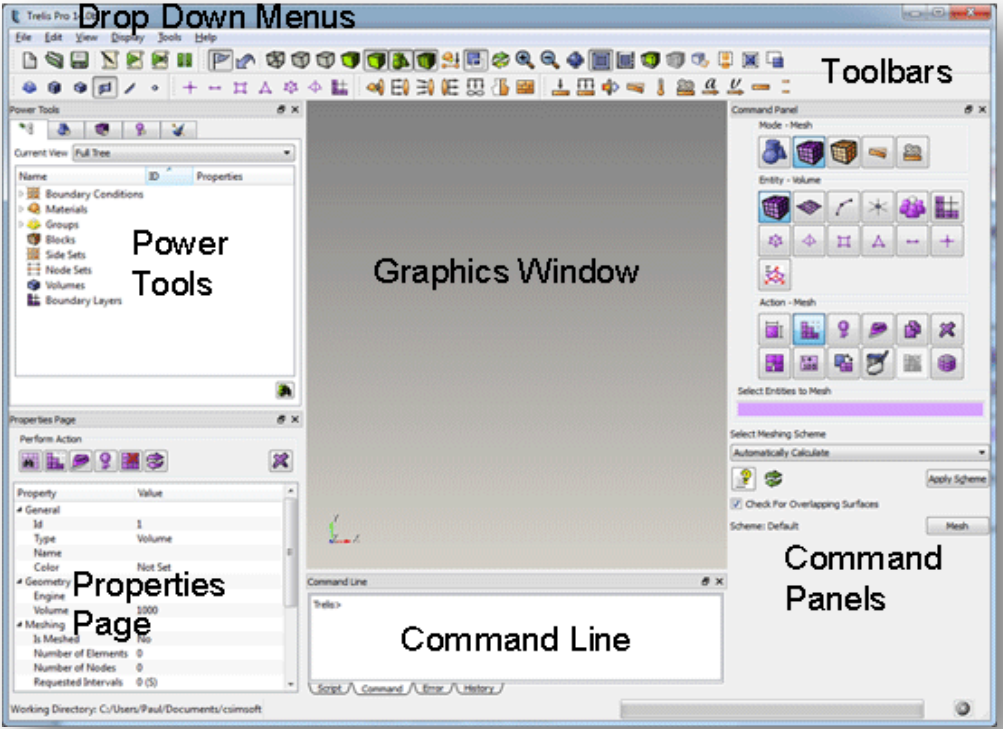
\includegraphics[trim=.1cm .25cm 2.0cm .4cm, clip=true, totalheight=.8\textheight]{figures/gui_window.png}
        \end{center}
\end{frame}

\begin{frame}
\frametitle{Create a simple mesh}
\begin{itemize}
 \item Creating the geometry
 \item Setting the interval sizes and meshing schemes
 \item Meshing the geometry
 \item Specifying the boundary conditions
 \item Exporting the mesh
\end{itemize}
\end{frame}

\begin{frame}
 \frametitle{Generated mesh for brick with cylindrical Hole}
 \begin{itemize}
  \item Step 1: Beginning Execution
  \item Step 2: Creating the Brick
  \item Step 3: Creating the Cylinder
  \item Step 4: Adjusting the Graphics Display
  \item Step 5: Forming the Hole
  \item Step 6: Setting Interval Sizes
  \item Step 7: Surface Meshing
  \item Step 8: Volume Meshing
  \item Step 9: Inspecting the Model
  \item Step 10: Materials and Boundary Conditions
  \item Step 11: Exporting the Mesh
 \end{itemize}
\end{frame}

\begin{frame}
 \frametitle{Generated mesh for brick with cylindrical Hole(Cont.)}

\begin{columns}[t]
\column{.33\textwidth}
\centering
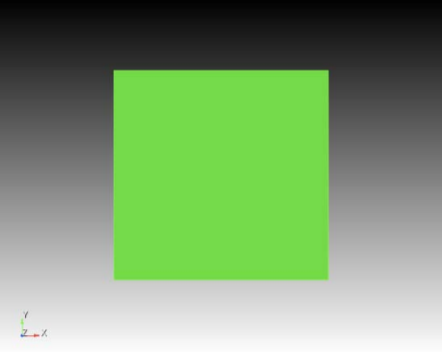
\includegraphics[width=3cm,height=2cm]{figures/step_2.png}\\

\includegraphics[width=3cm,height=2cm]{figures/step_3.png}\\
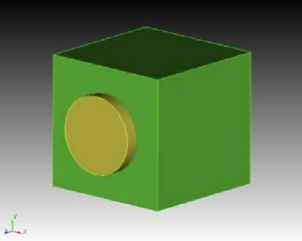
\includegraphics[width=3cm,height=2cm]{figures/step_4.png}
\column{.33\textwidth}
\centering
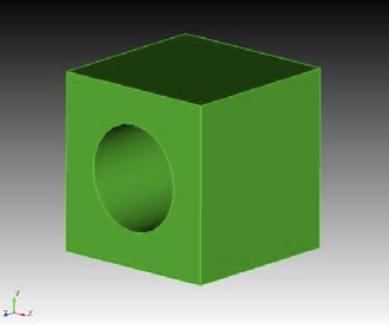
\includegraphics[width=3cm,height=2cm]{figures/step_5.png}\\
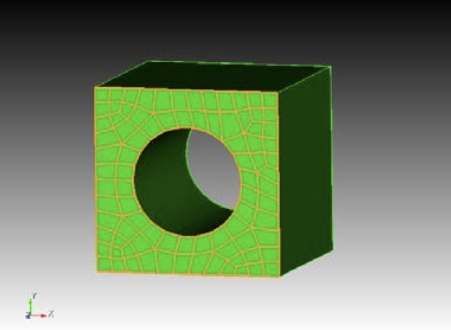
\includegraphics[width=3cm,height=2cm]{figures/step_7.png}\\
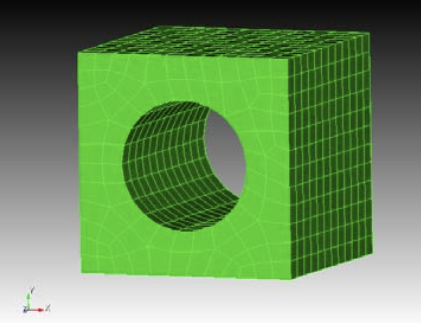
\includegraphics[width=3cm,height=2cm]{figures/step_8.png}\\
\column{.33\textwidth}
\centering
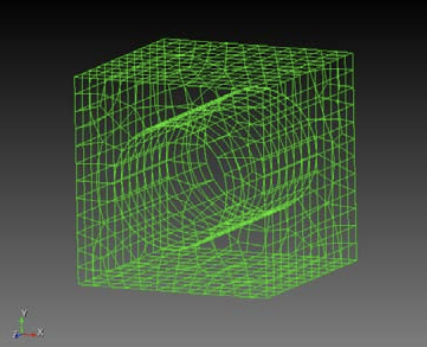
\includegraphics[width=3cm,height=2cm]{figures/step_9.png}\\
\end{columns}

\end{frame}
%%%%%%%%%%%%%%%%%%%%%%%%%%%%%%%%%%%%%%%%%%%%%%%%%%%%%%%%%%%%%%%%%%%%%%%%%%%
\section{Decomposition}
\begin{frame}
\frametitle{sweepable model}
\begin{block}{What volume is sweepable}
 Sweepable volumes can be comprised of many
different topologies. We typically classify sweeping problems into three groups, based on the number of
source/target surfaces.
\begin{itemize}
 \item One-to-one: A volume with a one source surface and one target surface.
 \item Many-to-one: A volume with multiple source surfaces and one target surface
 \item Multisweep (or Many-to-Many): A volume with multiple target surfaces
\end{itemize}
\end{block}
\end{frame}

\begin{frame}
 \frametitle{sweepable model}
 \begin{columns}[t]
\column{.33\textwidth}
\centering
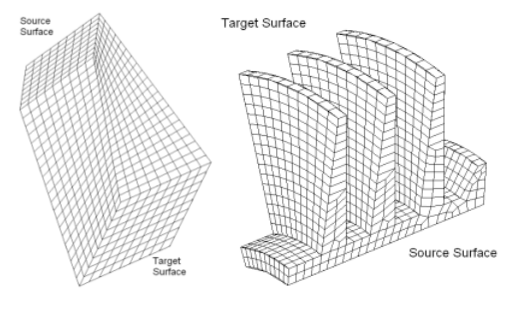
\includegraphics[width=4cm,height=3cm]{figures/one_to_one.png}\\{One to one}
\column{.33\textwidth}
\centering
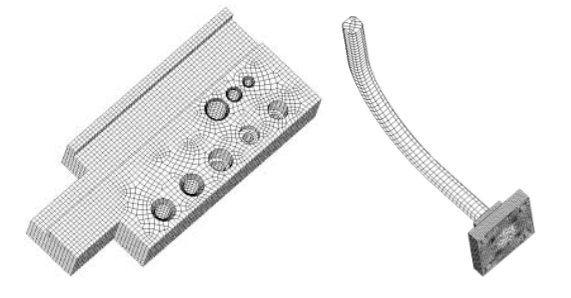
\includegraphics[width=4cm,height=3cm]{figures/many_to_one.png}\\{Many to one}
\column{.33\textwidth}
\centering
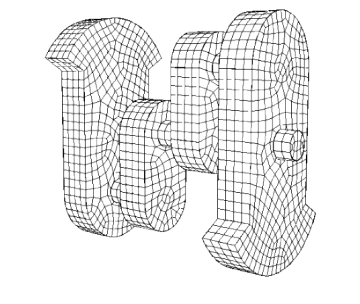
\includegraphics[width=4cm,height=3cm]{figures/many_to_many.png}\\{Many to many}
\end{columns}
\end{frame}












%%%%%%%%%%%%%%%%%%%%%%%%%%%%%%%%%%%%%%%%%%%%%%%%%%%%%%%%%%%%%%%%%%%%%%%%%%%
\end{document}
